\documentclass[10pt,a4paper,noindentfirst]{article}\usepackage[]{graphicx}\usepackage[]{color}
%% maxwidth is the original width if it is less than linewidth
%% otherwise use linewidth (to make sure the graphics do not exceed the margin)
\makeatletter
\def\maxwidth{ %
  \ifdim\Gin@nat@width>\linewidth
    \linewidth
  \else
    \Gin@nat@width
  \fi
}
\makeatother

\definecolor{fgcolor}{rgb}{0.345, 0.345, 0.345}
\newcommand{\hlnum}[1]{\textcolor[rgb]{0.686,0.059,0.569}{#1}}%
\newcommand{\hlstr}[1]{\textcolor[rgb]{0.192,0.494,0.8}{#1}}%
\newcommand{\hlcom}[1]{\textcolor[rgb]{0.678,0.584,0.686}{\textit{#1}}}%
\newcommand{\hlopt}[1]{\textcolor[rgb]{0,0,0}{#1}}%
\newcommand{\hlstd}[1]{\textcolor[rgb]{0.345,0.345,0.345}{#1}}%
\newcommand{\hlkwa}[1]{\textcolor[rgb]{0.161,0.373,0.58}{\textbf{#1}}}%
\newcommand{\hlkwb}[1]{\textcolor[rgb]{0.69,0.353,0.396}{#1}}%
\newcommand{\hlkwc}[1]{\textcolor[rgb]{0.333,0.667,0.333}{#1}}%
\newcommand{\hlkwd}[1]{\textcolor[rgb]{0.737,0.353,0.396}{\textbf{#1}}}%

\usepackage{framed}
\makeatletter
\newenvironment{kframe}{%
 \def\at@end@of@kframe{}%
 \ifinner\ifhmode%
  \def\at@end@of@kframe{\end{minipage}}%
  \begin{minipage}{\columnwidth}%
 \fi\fi%
 \def\FrameCommand##1{\hskip\@totalleftmargin \hskip-\fboxsep
 \colorbox{shadecolor}{##1}\hskip-\fboxsep
     % There is no \\@totalrightmargin, so:
     \hskip-\linewidth \hskip-\@totalleftmargin \hskip\columnwidth}%
 \MakeFramed {\advance\hsize-\width
   \@totalleftmargin\z@ \linewidth\hsize
   \@setminipage}}%
 {\par\unskip\endMakeFramed%
 \at@end@of@kframe}
\makeatother

\definecolor{shadecolor}{rgb}{.97, .97, .97}
\definecolor{messagecolor}{rgb}{0, 0, 0}
\definecolor{warningcolor}{rgb}{1, 0, 1}
\definecolor{errorcolor}{rgb}{1, 0, 0}
\newenvironment{knitrout}{}{} % an empty environment to be redefined in TeX

\usepackage{alltt}

\usepackage[T1]{fontenc}
\usepackage[polish]{babel}
\usepackage[cp1250]{inputenc}
\usepackage{amsmath}
\usepackage{amsfonts}
\usepackage{graphicx}
\usepackage{setspace}
\usepackage{savesym}
\savesymbol{arc}
\usepackage{color}
\usepackage{xcolor}
\usepackage{pict2e}
\usepackage{epstopdf}
\usepackage{geometry}

\newgeometry{tmargin=0.9cm, bmargin=0.9cm, lmargin=0.9cm, rmargin=0.9cm}
\pagestyle{empty}
\linespread{1.2}
\IfFileExists{upquote.sty}{\usepackage{upquote}}{}
\begin{document}

\begin{knitrout}
\definecolor{shadecolor}{rgb}{0.969, 0.969, 0.969}\color{fgcolor}\begin{kframe}
\begin{alltt}
\hlcom{# zad.1}

\hlkwd{library}\hlstd{(}\hlstr{"tseries"}\hlstd{)}

\hlcom{# a)}

\hlstd{xt} \hlkwb{<-} \hlkwd{numeric}\hlstd{(}\hlnum{1100}\hlstd{)}
\hlstd{zt} \hlkwb{<-} \hlkwd{rnorm}\hlstd{(}\hlnum{1100}\hlstd{)}
\hlstd{alfa0} \hlkwb{<-} \hlnum{0.1}
\hlstd{alfa1} \hlkwb{<-} \hlnum{0.5}
\hlstd{alfa2} \hlkwb{<-} \hlnum{0.2}

\hlstd{xt[}\hlnum{1}\hlopt{:}\hlnum{2}\hlstd{]} \hlkwb{<-} \hlkwd{rnorm}\hlstd{(}\hlnum{2}\hlstd{,}\hlnum{0}\hlstd{,alfa0}\hlopt{/}\hlstd{(}\hlnum{1}\hlopt{-}\hlstd{alfa1}\hlopt{-}\hlstd{alfa2))}

\hlstd{skwt} \hlkwb{<-} \hlkwd{numeric}\hlstd{(}\hlnum{1100}\hlstd{)}
\hlkwa{for}\hlstd{(i} \hlkwa{in} \hlnum{3}\hlopt{:}\hlnum{1100}\hlstd{)\{}
  \hlstd{skwt[i]} \hlkwb{<-} \hlstd{alfa0} \hlopt{+} \hlstd{alfa1}\hlopt{*}\hlstd{xt[i}\hlopt{-}\hlnum{1}\hlstd{]}\hlopt{^}\hlnum{2} \hlopt{+} \hlstd{alfa2}\hlopt{*}\hlstd{xt[i}\hlopt{-}\hlnum{2}\hlstd{]}\hlopt{^}\hlnum{2}
  \hlstd{xt[i]} \hlkwb{<-} \hlkwd{sqrt}\hlstd{(skwt[i])}\hlopt{*}\hlstd{zt[i]}
\hlstd{\}}

\hlstd{xt} \hlkwb{<-} \hlstd{xt[}\hlnum{101}\hlopt{:}\hlnum{1100}\hlstd{]}
\hlkwd{ts.plot}\hlstd{(xt)}
\end{alltt}
\end{kframe}

{\centering \includegraphics[width=\maxwidth]{figure/unnamed-chunk-11} 

}


\begin{kframe}\begin{alltt}
\hlkwd{acf}\hlstd{(xt)}
\end{alltt}
\end{kframe}

{\centering 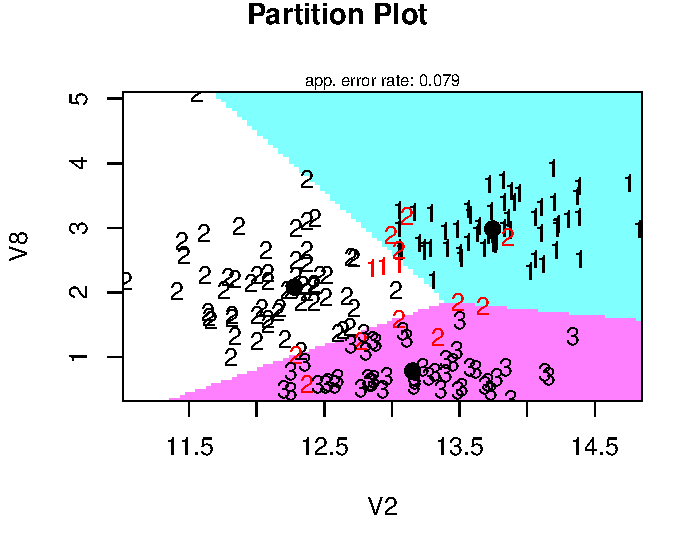
\includegraphics[width=\maxwidth]{figure/unnamed-chunk-12} 

}


\begin{kframe}\begin{alltt}
\hlcom{# b)}

\hlkwd{Box.test}\hlstd{(xt,}\hlkwc{lag}\hlstd{=}\hlnum{20}\hlstd{,}\hlkwc{type}\hlstd{=}\hlstr{"Ljung"}\hlstd{)}
\end{alltt}
\begin{verbatim}
## 
## 	Box-Ljung test
## 
## data:  xt
## X-squared = 19.78, df = 20, p-value = 0.4717
\end{verbatim}
\begin{alltt}
\hlcom{# nie wykrywa zaleznosci ARCH!!!!!!!! bo on wykrywa tylko zaleznosc linowa}
\hlkwd{Box.test}\hlstd{(xt}\hlopt{^}\hlnum{2}\hlstd{,}\hlkwc{lag}\hlstd{=}\hlnum{20}\hlstd{,}\hlkwc{type}\hlstd{=}\hlstr{"Ljung"}\hlstd{)}
\end{alltt}
\begin{verbatim}
## 
## 	Box-Ljung test
## 
## data:  xt^2
## X-squared = 146.7, df = 20, p-value < 2.2e-16
\end{verbatim}
\begin{alltt}
\hlcom{# a tu jest zaleznosc nielinowa! i tu juz wykrywa, dlatego, gdy chcemy spr,}
\hlcom{# czy jest efekt arch lub garch warto testowac kwadraty}

\hlcom{# c)}

\hlstd{mod} \hlkwb{<-} \hlkwd{arima}\hlstd{(xt}\hlopt{^}\hlnum{2}\hlstd{,}\hlkwd{c}\hlstd{(}\hlnum{2}\hlstd{,}\hlnum{0}\hlstd{,}\hlnum{0}\hlstd{))}
\hlkwd{Box.test}\hlstd{(mod}\hlopt{$}\hlstd{residuals,}\hlkwc{lag}\hlstd{=}\hlnum{20}\hlstd{,}\hlkwc{type}\hlstd{=}\hlstr{"Ljung"}\hlstd{)}
\end{alltt}
\begin{verbatim}
## 
## 	Box-Ljung test
## 
## data:  mod$residuals
## X-squared = 14.92, df = 20, p-value = 0.7808
\end{verbatim}
\begin{alltt}
\hlcom{# a teorerycznie powinien byc ar(2), wiec jest ok :D}

\hlcom{# d)}

\hlstd{arch} \hlkwb{<-} \hlkwd{garch}\hlstd{(xt,}\hlkwc{order}\hlstd{=}\hlkwd{c}\hlstd{(}\hlnum{0}\hlstd{,}\hlnum{2}\hlstd{),}\hlkwc{trace}\hlstd{=}\hlnum{FALSE}\hlstd{)}    \hlcom{# order(garch, arch) stopien}
\hlkwd{summary}\hlstd{(arch)}\hlopt{$}\hlstd{coef}   \hlcom{# mniej wiecej wychodza wartosci teoretyczne}
\end{alltt}
\begin{verbatim}
##     Estimate  Std. Error  t value Pr(>|t|)
## a0    0.1006     0.01021    9.851 0.00e+00
## a1    0.5675     0.06852    8.283 2.22e-16
## a2    0.1774     0.04238    4.187 2.83e-05
\end{verbatim}
\begin{alltt}
\hlcom{# e)}

\hlkwd{logLik}\hlstd{(arch)}  \hlcom{# logarytm wiarogodnosci}
\end{alltt}
\begin{verbatim}
## 'log Lik.' -692.1 (df=3)
\end{verbatim}
\begin{alltt}
\hlkwd{AIC}\hlstd{(arch)}
\end{alltt}
\begin{verbatim}
## [1] 1390
\end{verbatim}
\begin{alltt}
\hlcom{# f)}

\hlstd{fit} \hlkwb{<-} \hlkwd{fitted}\hlstd{(arch)}
\hlkwd{plot}\hlstd{(fit[,}\hlnum{1}\hlstd{]}\hlopt{^}\hlnum{2}\hlstd{,}\hlkwc{type}\hlstd{=}\hlstr{"l"}\hlstd{,}\hlkwc{ylab}\hlstd{=}\hlstr{"Conditional Variance"}\hlstd{)}
\end{alltt}
\end{kframe}

{\centering \includegraphics[width=\maxwidth]{figure/unnamed-chunk-13} 

}


\begin{kframe}\begin{alltt}
\hlcom{# wykres warunkowej wariancji}
\hlcom{# jaka mielismy wariancje w czasie t pod warunkiem wczesniejszego momentu}

\hlcom{# g)}

\hlstd{ga} \hlkwb{<-} \hlkwd{garch}\hlstd{(xt,}\hlkwc{order}\hlstd{=}\hlkwd{c}\hlstd{(}\hlnum{1}\hlstd{,}\hlnum{1}\hlstd{),}\hlkwc{trace}\hlstd{=}\hlnum{FALSE}\hlstd{)}
\hlkwd{summary}\hlstd{(ga)}
\end{alltt}
\begin{verbatim}
## 
## Call:
## garch(x = xt, order = c(1, 1), trace = FALSE)
## 
## Model:
## GARCH(1,1)
## 
## Residuals:
##      Min       1Q   Median       3Q      Max 
## -3.09777 -0.70481 -0.00749  0.67592  3.99037 
## 
## Coefficient(s):
##     Estimate  Std. Error  t value Pr(>|t|)    
## a0    0.0808      0.0125     6.46  1.1e-10 ***
## a1    0.5891      0.0733     8.03  8.9e-16 ***
## b1    0.2038      0.0576     3.54  0.00041 ***
## ---
## Signif. codes:  0 '***' 0.001 '**' 0.01 '*' 0.05 '.' 0.1 ' ' 1
## 
## Diagnostic Tests:
## 	Jarque Bera Test
## 
## data:  Residuals
## X-squared = 4.895, df = 2, p-value = 0.08653
## 
## 
## 	Box-Ljung test
## 
## data:  Squared.Residuals
## X-squared = 2.423, df = 1, p-value = 0.1196
\end{verbatim}
\begin{alltt}
\hlcom{# jaque bera test -> test na noramlnosc reziduow}
\hlcom{# ljunga boxa dla kwadratow reziduow}
\hlkwd{summary}\hlstd{(ga)}\hlopt{$}\hlstd{coef}
\end{alltt}
\begin{verbatim}
##     Estimate  Std. Error  t value  Pr(>|t|)
## a0   0.08079     0.01251    6.459 1.053e-10
## a1   0.58911     0.07333    8.033 8.882e-16
## b1   0.20378     0.05762    3.536 4.055e-04
\end{verbatim}
\begin{alltt}
\hlcom{# h)}

\hlkwd{AIC}\hlstd{(ga)}
\end{alltt}
\begin{verbatim}
## [1] 1396
\end{verbatim}
\begin{alltt}
\hlkwd{AIC}\hlstd{(arch)}
\end{alltt}
\begin{verbatim}
## [1] 1390
\end{verbatim}
\begin{alltt}
\hlcom{# lepszy jest ten, ktory ma mniejsza wartosc AIC}


\hlcom{# zad.3}

\hlcom{# O nieadekwatnosci modelowania zwrotow na}
\hlcom{# podstawie liniowych modeli autoregresyjnych}

\hlkwd{library}\hlstd{(}\hlstr{"evir"}\hlstd{)}

\hlkwd{data}\hlstd{(bmw,}\hlkwc{package}\hlstd{=}\hlstr{"evir"}\hlstd{)}
\hlcom{# bmw - wektor zwrotow logarytmicznych}

\hlkwd{head}\hlstd{(bmw)}
\end{alltt}
\begin{verbatim}
## [1]  0.047704  0.007127  0.008883 -0.012441 -0.003570  0.000000
\end{verbatim}
\begin{alltt}
\hlstd{bmw} \hlkwb{<-} \hlkwd{as.vector}\hlstd{(bmw)}
\hlstd{n} \hlkwb{<-} \hlkwd{length}\hlstd{(bmw)}

\hlkwd{acf}\hlstd{(bmw)}
\end{alltt}
\end{kframe}

{\centering \includegraphics[width=\maxwidth]{figure/unnamed-chunk-14} 

}


\begin{kframe}\begin{alltt}
\hlkwd{pacf}\hlstd{(bmw)}
\end{alltt}
\end{kframe}

{\centering \includegraphics[width=\maxwidth]{figure/unnamed-chunk-15} 

}


\begin{kframe}\begin{alltt}
\hlkwd{plot}\hlstd{(bmw)}
\end{alltt}
\end{kframe}

{\centering \includegraphics[width=\maxwidth]{figure/unnamed-chunk-16} 

}


\begin{kframe}\begin{alltt}
\hlkwa{for} \hlstd{(p} \hlkwa{in} \hlnum{0}\hlopt{:}\hlnum{3}\hlstd{) \{}
  \hlkwa{for} \hlstd{(q} \hlkwa{in} \hlnum{0}\hlopt{:}\hlnum{3}\hlstd{) \{}
    \hlstd{a} \hlkwb{<-} \hlkwd{AIC}\hlstd{(}\hlkwd{arima}\hlstd{(bmw,}\hlkwd{c}\hlstd{(p,}\hlnum{0}\hlstd{,q)),}\hlkwc{k}\hlstd{=}\hlkwd{log}\hlstd{(n))}
    \hlkwd{print}\hlstd{(}\hlkwd{c}\hlstd{(p,q,a))}
  \hlstd{\}}
\hlstd{\}}
\end{alltt}
\begin{verbatim}
## [1]      0      0 -34367
## [1]      0      1 -34401
## [1]      0      2 -34395
## [1]      0      3 -34386
## [1]      1      0 -34399
## [1]      1      1 -34395
## [1]      1      2 -34386
## [1]      1      3 -34378
## [1]      2      0 -34394
## [1]      2      1 -34386
## [1]      2      2 -34377
## [1]      2      3 -34369
## [1]      3      0 -34386
## [1]      3      1 -34378
## [1]      3      2 -34369
## [1]      3      3 -34361
\end{verbatim}
\begin{alltt}
\hlcom{# metoda na oko - minimum sugeruje model MA(1)}

\hlstd{fitMA1} \hlkwb{<-} \hlkwd{arima}\hlstd{(bmw,} \hlkwc{order} \hlstd{=} \hlkwd{c}\hlstd{(}\hlnum{0}\hlstd{,}\hlnum{0}\hlstd{,} \hlnum{1}\hlstd{))}

\hlkwd{Box.test}\hlstd{(fitMA1}\hlopt{$}\hlstd{resid,}\hlkwc{lag}\hlstd{=}\hlnum{20}\hlstd{,}\hlkwc{type}\hlstd{=}\hlstr{"Ljung"}\hlstd{)}
\end{alltt}
\begin{verbatim}
## 
## 	Box-Ljung test
## 
## data:  fitMA1$resid
## X-squared = 37.31, df = 20, p-value = 0.01074
\end{verbatim}
\begin{alltt}
\hlkwd{Box.test}\hlstd{(fitMA1}\hlopt{$}\hlstd{resid}\hlopt{^}\hlnum{2}\hlstd{,}\hlkwc{lag}\hlstd{=}\hlnum{20}\hlstd{,}\hlkwc{type}\hlstd{=}\hlstr{"Ljung"}\hlstd{)}  \hlcom{# wskazuje na szereg ARCH}
\end{alltt}
\begin{verbatim}
## 
## 	Box-Ljung test
## 
## data:  fitMA1$resid^2
## X-squared = 1274, df = 20, p-value < 2.2e-16
\end{verbatim}
\begin{alltt}
\hlkwd{acf}\hlstd{(} \hlkwd{residuals}\hlstd{(fitMA1),}\hlkwc{lag.max}\hlstd{=}\hlnum{20}\hlstd{)}
\end{alltt}
\end{kframe}

{\centering \includegraphics[width=\maxwidth]{figure/unnamed-chunk-17} 

}


\begin{kframe}\begin{alltt}
\hlkwd{qqnorm}\hlstd{(}\hlkwd{residuals}\hlstd{(fitMA1),}\hlkwc{datax}\hlstd{=T,}\hlkwc{main}\hlstd{=}\hlstr{"MA(1) resid"}\hlstd{)}
\end{alltt}
\end{kframe}

{\centering \includegraphics[width=\maxwidth]{figure/unnamed-chunk-18} 

}


\begin{kframe}\begin{alltt}
\hlkwd{plot}\hlstd{(}\hlkwd{residuals}\hlstd{(fitMA1),}\hlkwc{ylab}\hlstd{=}\hlstr{"Residual"}\hlstd{)}
\end{alltt}
\end{kframe}

{\centering \includegraphics[width=\maxwidth]{figure/unnamed-chunk-19} 

}


\begin{kframe}\begin{alltt}
\hlcom{# rozklad rezydu�w nie jest normalny}
\hlcom{# widoczne skupienia zmienno�ci => rezydua s� zale�ne}


\hlcom{# dopasowujemy model MA(1) + rezydua GARCH(1,1), rozklad warunkowy normalny}

\hlkwd{library}\hlstd{(}\hlstr{"fGarch"}\hlstd{)}

\hlstd{bmw.garch_norm} \hlkwb{<-} \hlkwd{garchFit}\hlstd{(}\hlopt{~}\hlkwd{arma}\hlstd{(}\hlnum{0}\hlstd{,}\hlnum{1}\hlstd{)}\hlopt{+}\hlkwd{garch}\hlstd{(}\hlnum{1}\hlstd{,}\hlnum{1}\hlstd{),} \hlkwc{data}\hlstd{=bmw,}
                          \hlkwc{cond.dist}\hlstd{=}\hlstr{"norm"}\hlstd{,}\hlkwc{trace}\hlstd{=}\hlnum{FALSE}\hlstd{)}
\hlcom{# dopasuje arma do danych a garch do residuow}
\hlkwd{summary}\hlstd{(bmw.garch_norm)}  \hlcom{# ljung box -> to Q() oznacza jaki lag}
\end{alltt}
\begin{verbatim}
## 
## Title:
##  GARCH Modelling 
## 
## Call:
##  garchFit(formula = ~arma(0, 1) + garch(1, 1), data = bmw, cond.dist = "norm", 
##     trace = FALSE) 
## 
## Mean and Variance Equation:
##  data ~ arma(0, 1) + garch(1, 1)
## <environment: 0x00000000091da668>
##  [data = bmw]
## 
## Conditional Distribution:
##  norm 
## 
## Coefficient(s):
##         mu         ma1       omega      alpha1       beta1  
## 4.4430e-04  1.0023e-01  8.9488e-06  1.0251e-01  8.5886e-01  
## 
## Std. Errors:
##  based on Hessian 
## 
## Error Analysis:
##         Estimate  Std. Error  t value Pr(>|t|)    
## mu     4.443e-04   1.738e-04    2.556   0.0106 *  
## ma1    1.002e-01   1.443e-02    6.946 3.76e-12 ***
## omega  8.949e-06   1.453e-06    6.160 7.28e-10 ***
## alpha1 1.025e-01   1.139e-02    9.003  < 2e-16 ***
## beta1  8.589e-01   1.585e-02   54.193  < 2e-16 ***
## ---
## Signif. codes:  0 '***' 0.001 '**' 0.01 '*' 0.05 '.' 0.1 ' ' 1
## 
## Log Likelihood:
##  17757    normalized:  2.889 
## 
## Description:
##  Wed Jun 11 13:07:39 2014 by user: Marta 
## 
## 
## Standardised Residuals Tests:
##                                 Statistic p-Value
##  Jarque-Bera Test   R    Chi^2  11330     0      
##  Shapiro-Wilk Test  R    W      NA        NA     
##  Ljung-Box Test     R    Q(10)  14.79     0.1398 
##  Ljung-Box Test     R    Q(15)  19.78     0.1806 
##  Ljung-Box Test     R    Q(20)  30.22     0.06643
##  Ljung-Box Test     R^2  Q(10)  5.054     0.8875 
##  Ljung-Box Test     R^2  Q(15)  7.528     0.9413 
##  Ljung-Box Test     R^2  Q(20)  9.264     0.9796 
##  LM Arch Test       R    TR^2   6.053     0.9134 
## 
## Information Criterion Statistics:
##    AIC    BIC    SIC   HQIC 
## -5.777 -5.771 -5.777 -5.775
\end{verbatim}
\begin{alltt}
\hlcom{# wykres kwantylowy dla rezydu�w}

\hlstd{x} \hlkwb{<-} \hlstd{bmw.garch_norm}\hlopt{@}\hlkwc{residuals} \hlopt{/} \hlstd{bmw.garch_norm}\hlopt{@}\hlkwc{sigma.t}
\hlkwd{plot}\hlstd{(x)}
\end{alltt}
\end{kframe}

{\centering \includegraphics[width=\maxwidth]{figure/unnamed-chunk-110} 

}


\begin{kframe}\begin{alltt}
\hlkwd{qqnorm}\hlstd{(x,}\hlkwc{datax}\hlstd{=T,}\hlkwc{ylab}\hlstd{=} \hlstr{"Standardized residual quantiles"}\hlstd{,}
       \hlkwc{main}\hlstd{=}\hlstr{" normal plot"}\hlstd{,} \hlkwc{xlab}\hlstd{=}\hlstr{"normal quantiles"}\hlstd{)}
\hlkwd{qqline}\hlstd{(x,}\hlkwc{datax}\hlstd{=T)}
\end{alltt}
\end{kframe}

{\centering \includegraphics[width=\maxwidth]{figure/unnamed-chunk-111} 

}


\begin{kframe}\begin{alltt}
\hlcom{# duze odstepstwa od normalnosci - grubsze ogony.}
\hlcom{# Dopasowujemy rozklad t do rezyduow.}
\hlcom{# Wykonujemy qqplot  dla rozkladu t o 4 st. sw.}

\hlstd{grid} \hlkwb{=} \hlstd{(}\hlnum{1}\hlopt{:}\hlstd{n)}\hlopt{/}\hlstd{(n}\hlopt{+}\hlnum{1}\hlstd{)}
\hlkwd{qqplot}\hlstd{(}\hlkwd{sort}\hlstd{(x),} \hlkwd{qt}\hlstd{(grid,}\hlkwc{df}\hlstd{=}\hlnum{4}\hlstd{),}
       \hlkwc{main}\hlstd{=} \hlstr{" t plot, df=4"}\hlstd{,}\hlkwc{xlab}\hlstd{=} \hlstr{"Standardized residual quantiles"}\hlstd{,}
       \hlkwc{ylab}\hlstd{=}\hlstr{"t-quantiles"}\hlstd{)}
\hlkwd{abline}\hlstd{(}   \hlkwd{lm}\hlstd{(}   \hlkwd{qt}\hlstd{(}\hlkwd{c}\hlstd{(}\hlnum{.25}\hlstd{,}\hlnum{.75}\hlstd{),}\hlkwc{df}\hlstd{=}\hlnum{4}\hlstd{)}\hlopt{~}\hlkwd{quantile}\hlstd{(x,}\hlkwd{c}\hlstd{(}\hlnum{.25}\hlstd{,}\hlnum{.75}\hlstd{))   )   )}
\end{alltt}
\end{kframe}

{\centering \includegraphics[width=\maxwidth]{figure/unnamed-chunk-112} 

}


\begin{kframe}\begin{alltt}
\hlcom{# zmieniamy rozklad warunkowy na t}

\hlstd{bmw.garch_t} \hlkwb{<-} \hlkwd{garchFit}\hlstd{(}\hlopt{~}\hlkwd{arma}\hlstd{(}\hlnum{0}\hlstd{,}\hlnum{1}\hlstd{)}\hlopt{+}\hlkwd{garch}\hlstd{(}\hlnum{1}\hlstd{,}\hlnum{1}\hlstd{),}\hlkwc{cond.dist}\hlstd{=}\hlstr{"std"}\hlstd{,}
                        \hlkwc{data}\hlstd{=bmw,}\hlkwc{trace}\hlstd{=}\hlnum{FALSE}\hlstd{)}

\hlkwd{options}\hlstd{(}\hlkwc{digits}\hlstd{=}\hlnum{4}\hlstd{)}
\hlkwd{summary}\hlstd{(bmw.garch_t)}  \hlcom{# parametr shape-> stopnie swobody.}
\end{alltt}
\begin{verbatim}
## 
## Title:
##  GARCH Modelling 
## 
## Call:
##  garchFit(formula = ~arma(0, 1) + garch(1, 1), data = bmw, cond.dist = "std", 
##     trace = FALSE) 
## 
## Mean and Variance Equation:
##  data ~ arma(0, 1) + garch(1, 1)
## <environment: 0x000000000a1aae90>
##  [data = bmw]
## 
## Conditional Distribution:
##  std 
## 
## Coefficient(s):
##         mu         ma1       omega      alpha1       beta1       shape  
## 1.3083e-04  6.8514e-02  6.0813e-06  9.3850e-02  8.8599e-01  4.0557e+00  
## 
## Std. Errors:
##  based on Hessian 
## 
## Error Analysis:
##         Estimate  Std. Error  t value Pr(>|t|)    
## mu     1.308e-04   1.439e-04    0.909    0.363    
## ma1    6.851e-02   1.293e-02    5.300 1.16e-07 ***
## omega  6.081e-06   1.349e-06    4.508 6.56e-06 ***
## alpha1 9.385e-02   1.322e-02    7.101 1.24e-12 ***
## beta1  8.860e-01   1.548e-02   57.223  < 2e-16 ***
## shape  4.056e+00   2.327e-01   17.428  < 2e-16 ***
## ---
## Signif. codes:  0 '***' 0.001 '**' 0.01 '*' 0.05 '.' 0.1 ' ' 1
## 
## Log Likelihood:
##  18158    normalized:  2.954 
## 
## Description:
##  Wed Jun 11 13:07:41 2014 by user: Marta 
## 
## 
## Standardised Residuals Tests:
##                                 Statistic p-Value
##  Jarque-Bera Test   R    Chi^2  13383     0      
##  Shapiro-Wilk Test  R    W      NA        NA     
##  Ljung-Box Test     R    Q(10)  21.38     0.01859
##  Ljung-Box Test     R    Q(15)  25.92     0.03889
##  Ljung-Box Test     R    Q(20)  36.18     0.01465
##  Ljung-Box Test     R^2  Q(10)  5.801     0.8317 
##  Ljung-Box Test     R^2  Q(15)  8.157     0.9173 
##  Ljung-Box Test     R^2  Q(20)  10.77     0.9519 
##  LM Arch Test       R    TR^2   7.008     0.8571 
## 
## Information Criterion Statistics:
##    AIC    BIC    SIC   HQIC 
## -5.907 -5.900 -5.907 -5.905
\end{verbatim}
\begin{alltt}
\hlstd{loglik_bmw} \hlkwb{<-} \hlstd{bmw.garch_t}\hlopt{@}\hlkwc{fit}\hlopt{$}\hlstd{llh} \hlcom{# -loglik dla modelu bmw.garch_t}

\hlstd{BIC_bmw_t} \hlkwb{<-} \hlnum{2}\hlopt{*}\hlstd{loglik_bmw}\hlopt{+}\hlkwd{log}\hlstd{(n)}\hlopt{*}\hlnum{6}
\hlkwd{as.numeric}\hlstd{(BIC_bmw_t)} \hlcom{# warto�� kryterium BIC dla tego modelu}
\end{alltt}
\begin{verbatim}
## [1] -36263
\end{verbatim}
\begin{alltt}
\hlcom{# lepiej (mniej) niz w modelu ma cos dopasowanym na poczatku tego zadania}

\hlcom{# zad.2}

\hlcom{# 1)}

\hlstd{x} \hlkwb{<-} \hlkwd{read.table}\hlstd{(}\hlstr{"http://gamma.mini.pw.edu.pl/~szymanowskih/lab6/exch1.txt"}\hlstd{)}
\hlkwd{head}\hlstd{(x,}\hlnum{2}\hlstd{)}
\end{alltt}
\begin{verbatim}
##       V1
## 1 -0.102
## 2  0.000
\end{verbatim}
\begin{alltt}
\hlkwd{ts.plot}\hlstd{(x)}
\end{alltt}
\end{kframe}

{\centering \includegraphics[width=\maxwidth]{figure/unnamed-chunk-113} 

}


\begin{kframe}\begin{alltt}
\hlkwd{acf}\hlstd{(x)}
\end{alltt}
\end{kframe}

{\centering \includegraphics[width=\maxwidth]{figure/unnamed-chunk-114} 

}


\begin{kframe}\begin{alltt}
\hlkwd{pacf}\hlstd{(x)}
\end{alltt}
\end{kframe}

{\centering \includegraphics[width=\maxwidth]{figure/unnamed-chunk-115} 

}


\begin{kframe}\begin{alltt}
\hlkwd{Box.test}\hlstd{(x,}\hlkwc{lag}\hlstd{=}\hlnum{20}\hlstd{,}\hlkwc{type}\hlstd{=}\hlstr{"Ljung"}\hlstd{)}
\end{alltt}
\begin{verbatim}
## 
## 	Box-Ljung test
## 
## data:  x
## X-squared = 32.24, df = 20, p-value = 0.04079
\end{verbatim}
\begin{alltt}
\hlkwd{Box.test}\hlstd{(x}\hlopt{^}\hlnum{2}\hlstd{,}\hlkwc{lag}\hlstd{=}\hlnum{20}\hlstd{,}\hlkwc{type}\hlstd{=}\hlstr{"Ljung"}\hlstd{)}
\end{alltt}
\begin{verbatim}
## 
## 	Box-Ljung test
## 
## data:  x^2
## X-squared = 94.2, df = 20, p-value = 1.356e-11
\end{verbatim}
\begin{alltt}
\hlcom{# te powyzsze testy to bardzo charakterystyczna rzecza dla efektu arch}
\hlcom{# dla zwyklych danych nic sie nie dzieje, a dla kwadratow jest juz problem}

\hlstd{xt} \hlkwb{<-} \hlkwd{as.numeric}\hlstd{(}\hlkwd{as.matrix}\hlstd{(x))}

\hlcom{# 2)}

\hlkwd{plot}\hlstd{(}\hlkwd{density}\hlstd{(xt))}
\hlkwd{curve}\hlstd{(}\hlkwd{dnorm}\hlstd{(x,}\hlkwd{mean}\hlstd{(xt),}\hlkwd{sd}\hlstd{(xt)),}\hlkwc{add}\hlstd{=T,}\hlkwc{col}\hlstd{=}\hlstr{"red"}\hlstd{)}
\end{alltt}
\end{kframe}

{\centering \includegraphics[width=\maxwidth]{figure/unnamed-chunk-116} 

}


\begin{kframe}\begin{alltt}
\hlcom{# 4)}

\hlkwa{for}\hlstd{(i} \hlkwa{in} \hlnum{0}\hlopt{:}\hlnum{3}\hlstd{)\{}
  \hlkwa{for}\hlstd{(j} \hlkwa{in} \hlnum{1}\hlopt{:}\hlnum{3}\hlstd{)\{}
    \hlstd{a} \hlkwb{<-} \hlkwd{AIC}\hlstd{(}\hlkwd{garch}\hlstd{(xt,}\hlkwc{order}\hlstd{=}\hlkwd{c}\hlstd{(i,j),}\hlkwc{trace}\hlstd{=}\hlnum{FALSE}\hlstd{),}\hlkwc{k}\hlstd{=}\hlkwd{log}\hlstd{(}\hlkwd{length}\hlstd{(xt)))}
    \hlkwd{print}\hlstd{(}\hlkwd{c}\hlstd{(i,j,a))}
  \hlstd{\}}
\hlstd{\}}
\end{alltt}
\begin{verbatim}
## [1]     0     1 -6845
## [1]     0     2 -6851
## [1]     0     3 -6901
## [1]     1     1 -6959
## [1]     1     2 -6947
## [1]     1     3 -6863
## [1]     2     1 -6977
## [1]     2     2 -6907
## [1]     2     3 -6927
## [1]     3     1 -6971
## [1]     3     2 -6956
## [1]     3     3 -6894
\end{verbatim}
\begin{alltt}
\hlcom{# szukam minimum}
\end{alltt}
\end{kframe}
\end{knitrout}

\end{document}
